\documentclass[12pt]{article}
\usepackage{amsfonts, epsfig}

\usepackage{graphicx}
\usepackage{fancyhdr}
\pagestyle{fancy}
\lfoot{\texttt{github.com/conorhoughton/COMS30127}}
\lhead{Computation Neuroscience - 6\_mp\_neurons (d) - Conor}
\rhead{\thepage}
\cfoot{}

\usepackage{graphicx}
\usepackage{pstricks}
\usepackage{listings}

\usepackage{tikz}

\usepackage{pgf}
\usepackage[utf8]{inputenc}
\usetikzlibrary{arrows,automata}
\usetikzlibrary{positioning}


\tikzset{
    state/.style={
           rectangle,
           rounded corners,
           draw=black, very thick,
           inner sep=2pt,
           text centered,
           },
}
\tikzset{
    on/.style={
           circle,
           draw=red, very thick,
           inner sep=2pt,
           fill=red!25,
           },
}


\tikzset{
    off/.style={
           circle,
           draw=blue, very thick,
           inner sep=2pt,
           text centered,
           },
}



\tikzset{
    neuron/.style={
           rectangle,
           rounded corners,
           draw=black, very thick,
           inner sep=2pt,
           text centered,
           },
}



\tikzset{
    area/.style={
           rectangle,
           draw=black, very thick,
           inner sep=2pt,
           text centered,
           },
}


\tikzset{
    gc/.style={
           rectangle,
           rounded corners,
           draw=red, very thick,
           inner sep=2pt,
           text centered,
           },
}


\tikzset{
    inh/.style={
           rectangle,
           rounded corners,
           draw=blue, very thick,
           inner sep=2pt,
           text centered,
           },
}



\tikzset{
    io/.style={
           rectangle,
           draw=green, very thick,
           inner sep=2pt,
           text centered,
           },
}



\begin{document}

\section*{McCulloch-Pitts neurons} 

The McCulloch Pitts neuron model, or Threshold Logic Unit, was
introduced in 1943 by Warren McCulloch and Walter Pitts as a
computational model of a neuronal network \cite{McCullochPitts1943}. Their thinking was that
neurons are joined to each other with connections of variable
strength; in the soma the inputs from other neurons are added up and
they determine the activity of the neuron in a non-linear way; they
also knew that neurons tend to ignore input up to some threshold value
before responding strongly. These properties they tried to include in
their model neurons.

Artificial neurons, of the sort used in artificial intelligence, are
described by a single dynamical variable, $x_i$ say for a neuron
labelled $i$; the value of $x_i$ is determined by the weighted input
from the other neurons:
\begin{equation}
x_i=\phi\left(\sum_j w_{ij} x_j-\theta_i\right)
\end{equation}
$\phi$ is an activation function, $\theta$ is a threshold and the
$w_{ij}$ are the connection strengths weighting the inputs from the
other neurons. The McCulloch Pitts neuron was the first example of an
artificial neuron and had a step function for $\phi$:
\begin{equation}
x_i=\left\{\begin{array}{ll}1&\sum_j w_{ij} x_j>\theta_i\\-1&\mbox{otherwise}\end{array}\right.
\end{equation}
Thus, the neuron has two states, it is in the on state, $x_i=1$ if the
weighted input exceeds a threshold $\theta_i$ and an off state,
$x_i=-1$ if it doesn't; the picture you might have of how this
corresponds to the brain is that \lq{}on\rq{} corresponds to rapid
spiking and \lq{}off\rq{} to spiking at a much lower rate. The
$w_{ij}$, the connection strengths, are like the synapse strengths, a
positive $w_{ij}$ is an excitatory synapse and negative, an
inhibitory; a given neurons have both negative and positive
out-going synapses, that is there is no restriction that says $w_{ij}$
always has the same sign for a given $j$, this is different from real
neurons where all the outgoing synapses from a given neuron are either
excitatory or inhibitory.

While it should be clear that this network has some of the properties,
very abstracted, of a neuronal network, it might not be so clear what
can be done with the neurons. When they were working, at the dawn of
the age of electronic computers, McCulloch and Pitts believed that
their neurons might form the natural unit in computer circuits, in
other words, they thought they might perform the role actually played
by logical circuits. In fact, it is still not clear if the artificial
neuron is or isn't the natural unit of computation in silicon since
they are a component in, for example, deep learning networks. In fact,
there are two major applications of McCulloch-Pitts neurons: the
perceptron and the Hopfield network; these two applications add a rule
for changing the connection strength to the original McCulloch-Pitts
neuron.

\subsubsection*{Perceptrons}

The perceptron is a machine that does supervised learning, that is, it
makes guesses, is told whether or not its guess is correct, and then
makes another guess. They were first discovered in 1957 by Frank
Rosenblatt \cite{Rosenblatt1958} and introduced to the world with great fanfare, it was
claimed that they would solve problems from object recognition to
consciousness: if you consider the perceptron as the forbearer of the
deep learning network, then perhaps we don't know if these claims will
be fulfilled, but we do know that the original perceptron proved quite
limited in artificial intelligence. It does, however, appear to
describe some neuronal processes, if we ignore the implementation
details.

Anyway, a perceptron is made of two layers of neurons, an input layer
and an output layer of McCulloch-Pitts neurons. For simplicity let's
assume the output layer
has a single neuron. Now, if the input is given by
$\textbf{x}=(x_1,x_2,\ldots,x_n)$ the output, $y$, is
\begin{equation}
y=\phi(r)
\end{equation}
where
\begin{equation}
r=\sum_j w_j x_j-\theta
\end{equation}
and $\phi$ here is the simple Heaviside-like activation function
described above. Now for a given input, if the actual value of the
output should be $d$ the error is $d-y$. The perceptron learning rule
is to change the $w_j$ weight by an amount proportional to the error
and how much $x_j$ was \lq{}to blame\rq{} for the error:
\begin{equation}
\delta w_j=\eta (d-y) x_j
\end{equation}
and
\begin{equation}
\delta \theta =  \eta (d-y)
\end{equation}
where $\eta$ is some small learning rate and
\begin{eqnarray}
w_j&\rightarrow& w_j+\delta w_j\cr
\theta&\rightarrow& \theta+\delta\theta
\end{eqnarray}
You can see how this might work, if $x_j$ was positive and $y$ was too
big, this would make $w_j$ smaller so in future $y$ would be smaller
when it had the same input. 

In fact, the perceptron can only solve problems with a linear
classifier: if we think of the $x_i$'s as parametrizing an
$n$-dimensional space then $\sum_iw_ix_i=\theta$ is a hyperplane in
that space, so a pattern $\textbf{x}$ is classified one way or the
other according to which side of that hyperplane it lies, see for example Fig.~\ref{fig:linear_classifier}. Thus, the
perceptron works only if there is a hyperplane dividing the data into
two, with one class of data on one side and one on the other. In fact,
if the data is linearly separable the perceptron is guaranteed to
converge to a solution which manages this separation. Now, as
illustrated in Fig.~\ref{fig:random_points}, there will not be a unique
hyper-plane separating the two classes and the perceptron won't,
typically, find what you might regard as the \lq{}best\rq{}
hyperplane, where by best you might mean the line that is, in some
sense, as far from the individual data points as possible; finding
that best hyperplane is the idea behind the support vector machine.


\begin{figure}
% GNUPLOT: LaTeX picture with Postscript
\begingroup
  \makeatletter
  \providecommand\color[2][]{%
    \GenericError{(gnuplot) \space\space\space\@spaces}{%
      Package color not loaded in conjunction with
      terminal option `colourtext'%
    }{See the gnuplot documentation for explanation.%
    }{Either use 'blacktext' in gnuplot or load the package
      color.sty in LaTeX.}%
    \renewcommand\color[2][]{}%
  }%
  \providecommand\includegraphics[2][]{%
    \GenericError{(gnuplot) \space\space\space\@spaces}{%
      Package graphicx or graphics not loaded%
    }{See the gnuplot documentation for explanation.%
    }{The gnuplot epslatex terminal needs graphicx.sty or graphics.sty.}%
    \renewcommand\includegraphics[2][]{}%
  }%
  \providecommand\rotatebox[2]{#2}%
  \@ifundefined{ifGPcolor}{%
    \newif\ifGPcolor
    \GPcolorfalse
  }{}%
  \@ifundefined{ifGPblacktext}{%
    \newif\ifGPblacktext
    \GPblacktexttrue
  }{}%
  % define a \g@addto@macro without @ in the name:
  \let\gplgaddtomacro\g@addto@macro
  % define empty templates for all commands taking text:
  \gdef\gplbacktext{}%
  \gdef\gplfronttext{}%
  \makeatother
  \ifGPblacktext
    % no textcolor at all
    \def\colorrgb#1{}%
    \def\colorgray#1{}%
  \else
    % gray or color?
    \ifGPcolor
      \def\colorrgb#1{\color[rgb]{#1}}%
      \def\colorgray#1{\color[gray]{#1}}%
      \expandafter\def\csname LTw\endcsname{\color{white}}%
      \expandafter\def\csname LTb\endcsname{\color{black}}%
      \expandafter\def\csname LTa\endcsname{\color{black}}%
      \expandafter\def\csname LT0\endcsname{\color[rgb]{1,0,0}}%
      \expandafter\def\csname LT1\endcsname{\color[rgb]{0,1,0}}%
      \expandafter\def\csname LT2\endcsname{\color[rgb]{0,0,1}}%
      \expandafter\def\csname LT3\endcsname{\color[rgb]{1,0,1}}%
      \expandafter\def\csname LT4\endcsname{\color[rgb]{0,1,1}}%
      \expandafter\def\csname LT5\endcsname{\color[rgb]{1,1,0}}%
      \expandafter\def\csname LT6\endcsname{\color[rgb]{0,0,0}}%
      \expandafter\def\csname LT7\endcsname{\color[rgb]{1,0.3,0}}%
      \expandafter\def\csname LT8\endcsname{\color[rgb]{0.5,0.5,0.5}}%
    \else
      % gray
      \def\colorrgb#1{\color{black}}%
      \def\colorgray#1{\color[gray]{#1}}%
      \expandafter\def\csname LTw\endcsname{\color{white}}%
      \expandafter\def\csname LTb\endcsname{\color{black}}%
      \expandafter\def\csname LTa\endcsname{\color{black}}%
      \expandafter\def\csname LT0\endcsname{\color{black}}%
      \expandafter\def\csname LT1\endcsname{\color{black}}%
      \expandafter\def\csname LT2\endcsname{\color{black}}%
      \expandafter\def\csname LT3\endcsname{\color{black}}%
      \expandafter\def\csname LT4\endcsname{\color{black}}%
      \expandafter\def\csname LT5\endcsname{\color{black}}%
      \expandafter\def\csname LT6\endcsname{\color{black}}%
      \expandafter\def\csname LT7\endcsname{\color{black}}%
      \expandafter\def\csname LT8\endcsname{\color{black}}%
    \fi
  \fi
  \setlength{\unitlength}{0.0500bp}%
  \begin{picture}(5760.00,4032.00)%
    \gplgaddtomacro\gplbacktext{%
      \csname LTb\endcsname%
      \put(1425,704){\makebox(0,0)[r]{\strut{}-4}}%
      \put(1425,1087){\makebox(0,0)[r]{\strut{}-3}}%
      \put(1425,1470){\makebox(0,0)[r]{\strut{}-2}}%
      \put(1425,1853){\makebox(0,0)[r]{\strut{}-1}}%
      \put(1425,2236){\makebox(0,0)[r]{\strut{} 0}}%
      \put(1425,2618){\makebox(0,0)[r]{\strut{} 1}}%
      \put(1425,3001){\makebox(0,0)[r]{\strut{} 2}}%
      \put(1425,3384){\makebox(0,0)[r]{\strut{} 3}}%
      \put(1425,3767){\makebox(0,0)[r]{\strut{} 4}}%
      \put(1557,484){\makebox(0,0){\strut{}-3}}%
      \put(2068,484){\makebox(0,0){\strut{}-2}}%
      \put(2578,484){\makebox(0,0){\strut{}-1}}%
      \put(3089,484){\makebox(0,0){\strut{} 0}}%
      \put(3599,484){\makebox(0,0){\strut{} 1}}%
      \put(4110,484){\makebox(0,0){\strut{} 2}}%
      \put(4620,484){\makebox(0,0){\strut{} 3}}%
      \put(919,2235){\rotatebox{-270}{\makebox(0,0){\strut{}$y_1$}}}%
      \put(3088,154){\makebox(0,0){\strut{}$x_1$}}%
    }%
    \gplgaddtomacro\gplfronttext{%
    }%
    \gplbacktext
    \put(0,0){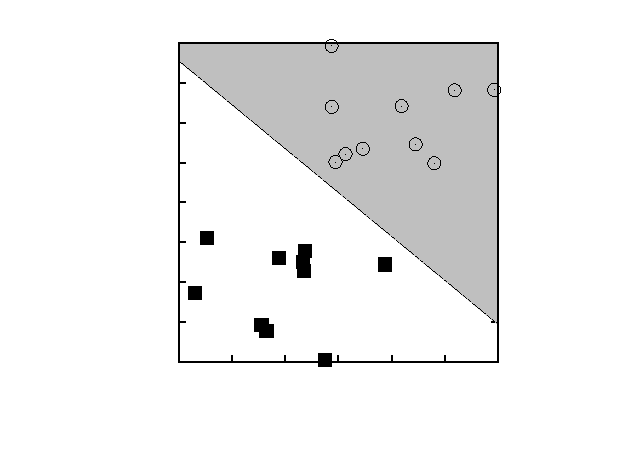
\includegraphics{linear_classifier}}%
    \gplfronttext
  \end{picture}%
\endgroup

\caption{Here the shaded region corresponds to $1.1x_1+x_2>0.25$, so
  if $w_1=1.1$ and $w_2=1$ with $\theta=0.25$ then the corresponding
  perceptron neuron will be one for all the circle points and -1 for
  all the square points.\label{fig:linear_classifier}}
\end{figure}


\begin{figure}
% GNUPLOT: LaTeX picture with Postscript
\begingroup
  \makeatletter
  \providecommand\color[2][]{%
    \GenericError{(gnuplot) \space\space\space\@spaces}{%
      Package color not loaded in conjunction with
      terminal option `colourtext'%
    }{See the gnuplot documentation for explanation.%
    }{Either use 'blacktext' in gnuplot or load the package
      color.sty in LaTeX.}%
    \renewcommand\color[2][]{}%
  }%
  \providecommand\includegraphics[2][]{%
    \GenericError{(gnuplot) \space\space\space\@spaces}{%
      Package graphicx or graphics not loaded%
    }{See the gnuplot documentation for explanation.%
    }{The gnuplot epslatex terminal needs graphicx.sty or graphics.sty.}%
    \renewcommand\includegraphics[2][]{}%
  }%
  \providecommand\rotatebox[2]{#2}%
  \@ifundefined{ifGPcolor}{%
    \newif\ifGPcolor
    \GPcolorfalse
  }{}%
  \@ifundefined{ifGPblacktext}{%
    \newif\ifGPblacktext
    \GPblacktexttrue
  }{}%
  % define a \g@addto@macro without @ in the name:
  \let\gplgaddtomacro\g@addto@macro
  % define empty templates for all commands taking text:
  \gdef\gplbacktext{}%
  \gdef\gplfronttext{}%
  \makeatother
  \ifGPblacktext
    % no textcolor at all
    \def\colorrgb#1{}%
    \def\colorgray#1{}%
  \else
    % gray or color?
    \ifGPcolor
      \def\colorrgb#1{\color[rgb]{#1}}%
      \def\colorgray#1{\color[gray]{#1}}%
      \expandafter\def\csname LTw\endcsname{\color{white}}%
      \expandafter\def\csname LTb\endcsname{\color{black}}%
      \expandafter\def\csname LTa\endcsname{\color{black}}%
      \expandafter\def\csname LT0\endcsname{\color[rgb]{1,0,0}}%
      \expandafter\def\csname LT1\endcsname{\color[rgb]{0,1,0}}%
      \expandafter\def\csname LT2\endcsname{\color[rgb]{0,0,1}}%
      \expandafter\def\csname LT3\endcsname{\color[rgb]{1,0,1}}%
      \expandafter\def\csname LT4\endcsname{\color[rgb]{0,1,1}}%
      \expandafter\def\csname LT5\endcsname{\color[rgb]{1,1,0}}%
      \expandafter\def\csname LT6\endcsname{\color[rgb]{0,0,0}}%
      \expandafter\def\csname LT7\endcsname{\color[rgb]{1,0.3,0}}%
      \expandafter\def\csname LT8\endcsname{\color[rgb]{0.5,0.5,0.5}}%
    \else
      % gray
      \def\colorrgb#1{\color{black}}%
      \def\colorgray#1{\color[gray]{#1}}%
      \expandafter\def\csname LTw\endcsname{\color{white}}%
      \expandafter\def\csname LTb\endcsname{\color{black}}%
      \expandafter\def\csname LTa\endcsname{\color{black}}%
      \expandafter\def\csname LT0\endcsname{\color{black}}%
      \expandafter\def\csname LT1\endcsname{\color{black}}%
      \expandafter\def\csname LT2\endcsname{\color{black}}%
      \expandafter\def\csname LT3\endcsname{\color{black}}%
      \expandafter\def\csname LT4\endcsname{\color{black}}%
      \expandafter\def\csname LT5\endcsname{\color{black}}%
      \expandafter\def\csname LT6\endcsname{\color{black}}%
      \expandafter\def\csname LT7\endcsname{\color{black}}%
      \expandafter\def\csname LT8\endcsname{\color{black}}%
    \fi
  \fi
  \setlength{\unitlength}{0.0500bp}%
  \begin{picture}(5760.00,4032.00)%
    \gplgaddtomacro\gplbacktext{%
      \csname LTb\endcsname%
      \put(1425,704){\makebox(0,0)[r]{\strut{}-6}}%
      \put(1425,1215){\makebox(0,0)[r]{\strut{}-4}}%
      \put(1425,1725){\makebox(0,0)[r]{\strut{}-2}}%
      \put(1425,2236){\makebox(0,0)[r]{\strut{} 0}}%
      \put(1425,2746){\makebox(0,0)[r]{\strut{} 2}}%
      \put(1425,3257){\makebox(0,0)[r]{\strut{} 4}}%
      \put(1425,3767){\makebox(0,0)[r]{\strut{} 6}}%
      \put(1557,484){\makebox(0,0){\strut{}-3}}%
      \put(2068,484){\makebox(0,0){\strut{}-2}}%
      \put(2578,484){\makebox(0,0){\strut{}-1}}%
      \put(3089,484){\makebox(0,0){\strut{} 0}}%
      \put(3599,484){\makebox(0,0){\strut{} 1}}%
      \put(4110,484){\makebox(0,0){\strut{} 2}}%
      \put(4620,484){\makebox(0,0){\strut{} 3}}%
      \put(919,2235){\rotatebox{-270}{\makebox(0,0){\strut{}$x_2$}}}%
      \put(3088,154){\makebox(0,0){\strut{}$x_1$}}%
    }%
    \gplgaddtomacro\gplfronttext{%
    }%
    \gplbacktext
    \put(0,0){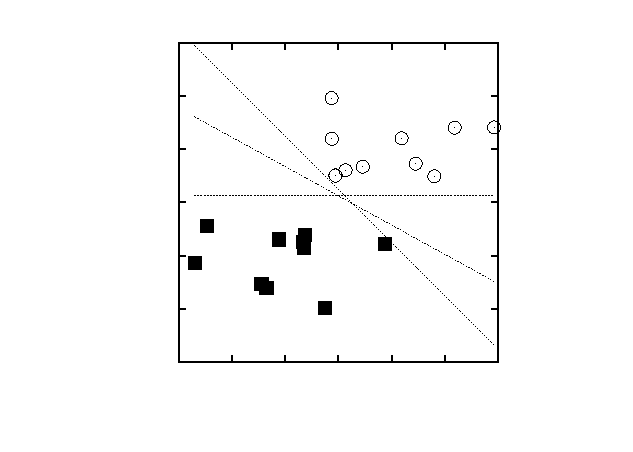
\includegraphics{random_points}}%
    \gplfronttext
  \end{picture}%
\endgroup

\caption{All of these lines separate the points into two classes\label{fig:random_points}}
\end{figure}

The perceptron learning rule can be motivated by thinking about error
minimization. Consider an error function
\begin{equation}
E=\langle(d^a-y^a)^2\rangle_a
\end{equation}
If $a$ labels lots of input, $\textbf{x}^a$, desired output $d^a$
pairs, with $y^a$ the actual output; the angle brackets are an average
over these pairs. Now consider the gradient of $E$ with $w_{i}$:
\begin{equation}
\frac{\partial E}{\partial w_{i}}=-2\left\langle (d^a-y_a) \frac{\partial y^a}{\partial w_{i}}\right\rangle
\end{equation}
Now if we ignore for the moment the fact that the activation function for the McCulloch-Pitt neuron isn't differentiable and write
\begin{equation}
y^=\phi(r)
\end{equation}
with 
\begin{equation}
r=\sum_{i}w_i x_i-\theta
\end{equation}
we have
\begin{equation}
\frac{dy^a}{dw_i}=\frac{d\phi}{dr}\frac{\partial r}{\partial w_i}
\end{equation}
so using
\begin{equation}
\frac{\partial r}{\partial w_i}=x_i
\end{equation}
we get
\begin{equation}
\frac{\partial E}{\partial w_{i}}=-2\left\langle (d^a-y^a)x^a_i (\mbox{stuff involving the derivative of }\phi)\right\rangle
\end{equation}
Of course, in the McCulloch-Pitts case the \lq{}stuff involving the
derivative of $\phi$\rq{} is either zero or undefined, but we can that
this gives a similar learning rule: one way to reduce the error is to
move a tiny amount in the opposite direction to the gradient, the
gradient is the direction along which the value increases
quickest. The actual perceptron rule we gave updates a small bit after
every presentation rather than averaging first over a collection of
presentations, both approaches make sense. Here we have dealt with the
weights, the same approach can be applied to the threshold $\theta$.

This is the way to a more modern approach to the perceptron rule and
these days smooth, or mostly-smooth activation functions are used in
artificial neurons for this reason. The basic limitation of the
perceptron is that it has only one layer and so only learns a linear
classification; these days artificial neural networks have more than
one layer; this complicates the idea of adjusting the $w_i$ in a way
that is weighted by $x_i$, this, in a sense, changing the weight
according to how much it is \lq{}to blame\rq{} for the error. Back
propagation resolves this, it can be thought of as propagating the
error backwards from layer to layer; although another way to think of
it is as doing gradient descent on all the weights. At the moment the
back propagation algorithm is not considered very biological, though
it is very possible that when we understand why deep learning networks
are so effective it will be clear that the important aspects of the
algorithm can be recognized in neuronal dynamics.

\subsection*{The cerebellum as a perceptron}

The cerebellum has a number of striking features; it has a more
stereotypical structure than most brain area and this structure is
conserved across species. It also has one of the brain's largest cells,
the Purkinje cell, and its most numerous, the granule cell.

\begin{figure}
\begin{center}
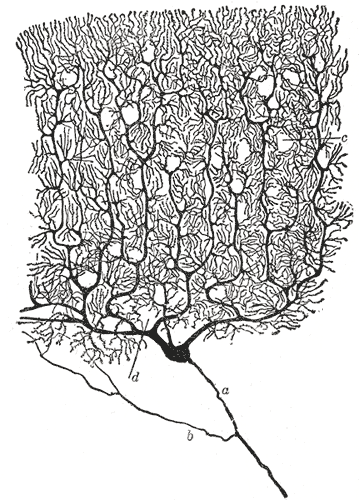
\includegraphics[width=7cm]{Purkinje_cell_by_Cajal.png}
\end{center}
\caption{A drawing by Santiago Ram\'{o}n y Cajal of a Purkinje cell. [Picture taken from \texttt{http://en.wikipedia.org/wiki/Golgi's\_method}]\label{fig:PC}}
\end{figure}

Purkinje cells have a distinctive structure with a huge, highly
branched, but flat dendritic arbor, see Fig.~\ref{fig:PC}; this allows
an extensive connectivity with each Purkinje cell receiving inputs
from around 100,000 other cells. In the cerebellum the Purkinje cell
are lined up like pages in a book, with their arbors lying in parallel
planes. They receive two excitatory inputs, weak inputs from parallel
fibres, axons that run perpendicular to the planes of the Purkinje
cell dendritic arbors, and a strong input from a climbing fibre, a
single axon which winds around the Purkinje cell and makes multiple
contacts with it, see Fig.~\ref{fig:cerebellum}.

\begin{figure}
\begin{center}
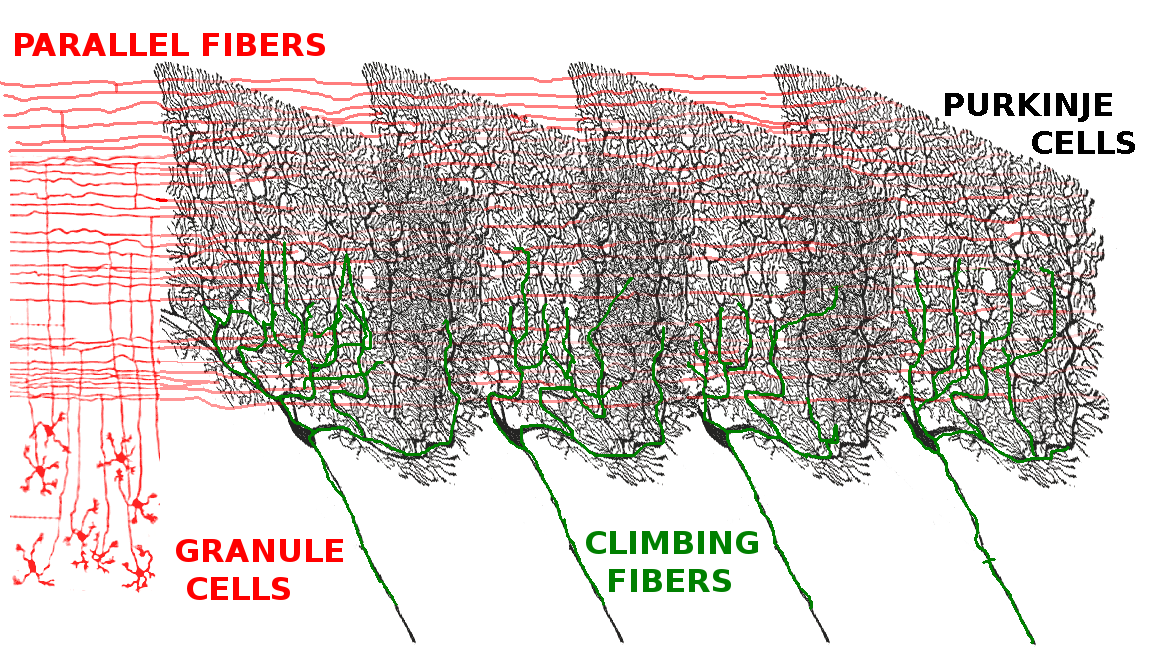
\includegraphics[width=11cm]{cerebellum.png}
\end{center}
\caption{A cartoon of the cerebellar circuitry. A vertical axon rises
  from each granule cells, splits once and then extends horizontally
  in two directions making connections with multiple Purkinje
  cells. Each Purkinje cell has its own climbing fiber which winds up
  around it.\label{fig:cerebellum}}
\end{figure}

\begin{figure}
\begin{center}
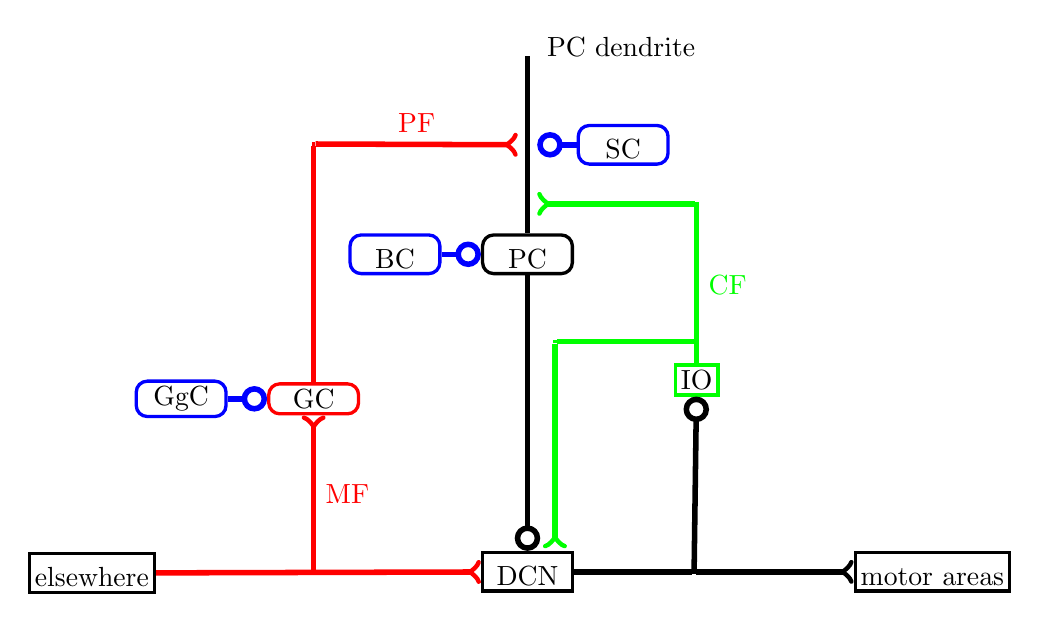
\begin{tikzpicture}
\node[neuron,text width=1cm, text height=0.35cm](PC){PC};
\node[inh,text width=1cm, text height=0.35cm,left = 0.5cm of PC](BC){BC};
\node[above = 1cm of PC](PCd){};
\node[inh,text width=1cm, text height=0.35cm,right = 0.5cm of PCd](SC){SC};
\node[above = 0.25cm of PC](PCc){};
\node[scale = 0.2,fill=green,right = 2cm of PCc](PCcr){};
\node[above = 1cm of PCd](PCdd){};
\node[right = 0cm of PCdd](){PC dendrite};
\node[left = 2cm of PC](PCl){};
\node[gc,text width=1cm,below = 1.5cm of PCl](GC){GC};
\node[inh,text width=1cm,left = 0.5cm of GC](GgC){GgC};
\node[scale = 0.2,fill=red,above = 3cm of GC](GCa){};
\node[scale = 0.01,fill=red,below = 2cm of GC](GCb){};
\node[io,below = 2cm of PCcr](IO){IO};
\node[scale =0.2,fill=green,above = 0.25cm of IO](IOa){};
\node[scale =0.2,fill=green,left = 1.75cm of IOa](IOl){};
\node[scale =0.01,below = 2.6cm of IOl](IOlb){};
\node[area,text width=1cm, text height=0.35cm,below  = 3.5cm of PC](DCN){DCN};
\node[scale=0.2,fill=black,right= 1.5cm of DCN](DCNr){};
\node[area,text height=0.35cm,right = 2cm of DCNr](ma){motor areas};
\node[area,text height=0.35cm,left = 2cm of GCb](ew){elsewhere};
\path (PCdd) edge[-,line width=2pt](PC);
\path (PC) edge[-o,line width=2pt] (DCN);
\path (IO) edge[-,green,line width=2pt] node[anchor=west]{CF} (PCcr);
\path (PCcr) edge[-<,green,line width=2pt] (PCc);
\path (GC) edge[-,red,line width=2pt] (GCa);
\path (GCa) edge[-<,red,line width=2pt] node[anchor=south]{PF}(PCd);
\path (GCb) edge[-<,red,line width=2pt] node[anchor=west]{MF} (GC);
\path (ew) edge[-<,red,line width=2pt] (DCN);
\path (DCN) edge[-,black,line width=2pt] (DCNr);
\path (DCNr) edge[-o,black,line width=2pt] (IO);
\path (DCNr) edge[-<,black,line width=2pt] (ma);
\path (IOa) edge[-,green,line width=2pt](IOl);
\path (IOl) edge[-<,green, line width=2pt](IOlb);
\path (GgC) edge[-o,blue, line width=2pt](GC);
\path (BC) edge[-o,blue, line width=2pt](PC);
\path (SC) edge[-o,blue, line width=2pt](PCd);
\end{tikzpicture}
\end{center}
\caption{A schematic of the cerebellar circuit. The granule cells (GC)
  receive input from a diverse range of other parts of the brain along
  the mossy fibers (MF). Each granule cell will combine input from
  just three or four mossy fibers and do this in lots of different
  combinations. The parallel fiber (PF) carries spikes from the GC to
  the Purkinje cell (PC) whose large dendrite is drawn as a line. The
  PC also receives input from a climbing fiber (CF) coming from
  Inferior Olivary Nucleus (IO). In turn it sends an inhibitory signal
  to the Deep Cerebellar Nucleus (DCN); the DCN has inhibitory neurons
  which act on IO and excitatory neurons which act on the motor
  system. The basket cells (BC), the Golgi cells (GgC) and the
  stellate cells (SC) are all local inhibitory
  cells.\label{fig:connectivity}}
\end{figure}

Another peculiarity is that the Purkinje cell has different responses
to different inputs; in response to multiple weak inputs from the
parallel fibers it fires a normal sort of spike, called in this
context a \textsl{simple spike}; in response to single spike from the
climbing fiber is fires a special spike, called a \textsl{complex
  spike}, with a leading spike, a number of small \lq{}spikelets\rq{}
and a sustained after-period of depolarization; this is illustrated in
Fig.~\ref{fig:spikes}.

\begin{figure}
\begin{center}
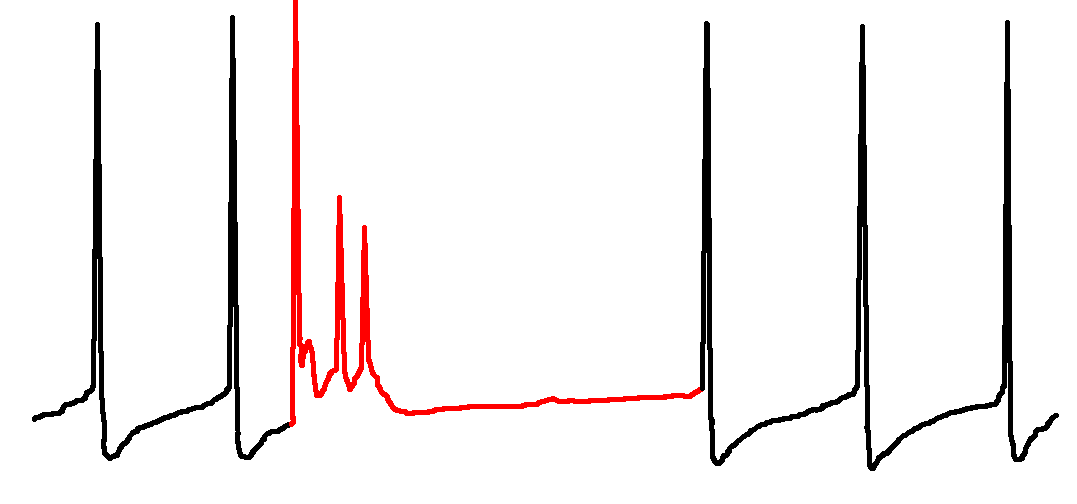
\includegraphics[width=8.cm]{complex_spike.png}
\end{center}
\caption{A complex spike. This drawing shows simple spikes in black
  and a complex spike in red. The complex spike is followed by a long
  refractory period during which spiking is not possible. This is a
  sketch, not an actual recording, but a typical time scale would have
  this refractory period 50 ms long.\label{fig:spikes}}
\end{figure}

It is still unclear exactly what the cerebellum does; what is known is
that it is important for actions, fine motor control and
proprioception; problems with the cerebellum are associated with
ataxia, loss of fine motor control, poor motor learning and poor
balance. There is a specific gait associated with cerebellar damage,
one that exhibits a certain self-consciousness or vigilance is
required for movement. According to most ideas about cerebellar
function it is required for the calculation of fine motor signals
\cite{Albus1971a}, or for predicting the sensory or proprioceptive
consequences of motor actions \cite{GaoEtAl1996a}; it is believed it
encodes forward and backwards models of movement so that it predicts
the consequences of motor commands, or calculates the motor command
that will a particular movement.

Whatever exactly it does, it is widely believed, in accordance with
the Marr-Albus model \cite{Marr1969a,Albus1971a}, that the connections
from parallel fibers to Purkinje cells acts as a perceptron. Thus, if
$y$ is the output of the Purkinje cell and, in this simple model,
taking into account the fact Purkinje cells are inhibitory
\begin{equation}
y=-\sum{w_ix_i}
\end{equation}
where the $x_i$s are the activities in the parallel fibers and $w_i$
is the strength of the synapse from the $i$th parallel fiber to the
Purkinje cell. The idea in the Marr-Albus model is that the climbing
fiber carries the error signal $d-y$ making the cerebellum an example
of supervised learning.

\subsection*{Hopfield network}

In contrast to a perceptron, a Hopfield network is a recurrently
connected network; it is intended to perform pattern completion and
was proposed by John Hopfield in 1982 \cite{Hopfield1982}, though other people had had the
idea before in different contexts. The idea behind a Hopfield network
is that you evolve the network according to the McCulloch-Pitts
relation, so, in the synchronous update version, from one iteration to
the next
\begin{equation}
\hat{x}_i=\phi\left(\sum_j w_{ij} x_j\right)
\end{equation}
and then $x_i\rightarrow \hat{x}$; that is all the nodes update using
the old values. In the most common version of a Hopfield network, the $w_{ij}$ are symmetric, that is
\begin{equation}
w_{ij}=w_{ji}
\end{equation}
The threshold values $\theta_i$ have been set to zero, this is
something you can do in a Hopfield network if you want because the
learning rule doesn't change to threshold. In the asynchronous scheme,
the you update the nodes one-by-one, for example, after choosing a
random node.


The idea is that this is a model for \textsl{auto-associative}
memory. Auto-associative memories are patterns representing memories
along with some dynamics that complete partial patters. Imagine a
sequence of McCulloch-Pitts neurons
\begin{center}

\begin{tikzpicture}
\filldraw[color=red!60, fill=red!25, very thick](0,0) circle (.25);
\filldraw[color=blue!60, fill=red!0, very thick](1,0) circle (.25);
\filldraw[color=red!60, fill=red!25, very thick](2,0) circle (.25);
\filldraw[color=blue!60, fill=red!0, very thick](3,0) circle (.25);
\filldraw[color=blue!60, fill=red!0, very thick](4,0) circle (.25);
\filldraw[color=red!60, fill=red!25, very thick](5,0) circle (.25);
\filldraw[color=blue!60, fill=red!0, very thick](6,0) circle (.25);
\filldraw[color=blue!60, fill=red!0, very thick](7,0) circle (.25);
\filldraw[color=blue!60, fill=red!0, very thick](8,0) circle (.25);
\end{tikzpicture}
\end{center}
where the filled circles correspond to on. Recall occurs when the
network is presented with a partial pattern and evolves into the
complete patterns.
\begin{center}
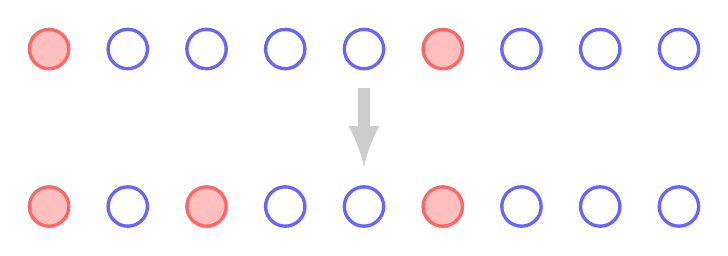
\begin{tikzpicture}
\filldraw[color=red!60, fill=red!25, very thick](0,2) circle (.25);
\filldraw[color=blue!60, fill=red!0, very thick](1,2) circle (.25);
\filldraw[color=blue!60, fill=red!0, very thick](2,2) circle (.25);
\filldraw[color=blue!60, fill=red!0, very thick](3,2) circle (.25);
\filldraw[color=blue!60, fill=red!0, very thick](4,2) circle (.25);
\filldraw[color=red!60, fill=red!25, very thick](5,2) circle (.25);
\filldraw[color=blue!60, fill=red!0, very thick](6,2) circle (.25);
\filldraw[color=blue!60, fill=red!0, very thick](7,2) circle (.25);
\filldraw[color=blue!60, fill=red!0, very thick](8,2) circle (.25);
\coordinate (a) at (4,1.5);
\coordinate (b) at (4,0.5);
\draw[->, >=latex, black!20!white, line width=4pt]   (a) to (b) ;
\filldraw[color=red!60, fill=red!25, very thick](0,0) circle (.25);
\filldraw[color=blue!60, fill=red!0, very thick](1,0) circle (.25);
\filldraw[color=red!60, fill=red!25, very thick](2,0) circle (.25);
\filldraw[color=blue!60, fill=red!0, very thick](3,0) circle (.25);
\filldraw[color=blue!60, fill=red!0, very thick](4,0) circle (.25);
\filldraw[color=red!60, fill=red!25, very thick](5,0) circle (.25);
\filldraw[color=blue!60, fill=red!0, very thick](6,0) circle (.25);
\filldraw[color=blue!60, fill=red!0, very thick](7,0) circle (.25);
\filldraw[color=blue!60, fill=red!0, very thick](8,0) circle (.25);
\end{tikzpicture}
\end{center}
The Hopfield network is intended to model the recall, and learning, of
memories in an autoassociative network.

One way to think about this is to note that there is an
\lq{}energy\rq{} associated with a Hopfield network:
\begin{equation}
E=-\frac{1}{2}\sum_{ij} w_{ij}x_ix_j
\end{equation}
and you can show than if you update a node you will reduce the energy.
Roughly speaking if you update a node $x_i$ then it is more likely to
have the same sign as a connected node $x_j$ if the connection between
them is large and positive since this means $w_{ij}x_j$ will have a
big effect on the activation of $x_i$ and vice versa; $x_i$ and $x_j$
are more likely to have an opposite sign if the connection is large
and negative. This means that updating the neurons will tend to reduce
the energy. In fact, this can be proved and that the system will
evolve to a local minimum.

Now the question is how to create the local minima? Here is a rules to
achieve this:
\begin{equation}
w_{ij}=\frac{1}{N}\sum_a x^a_ix^a_j
\end{equation}
where $N$ is the number of patterns to be stored, and $a$ indexes the
patterns. There are other rules, in fact there are rules that can
store more patterns, but rule, a sort of \lq{}top down\rq{} rule is
inspired by Hebbian plasticity. There is an online rule that is even
closer to Hebbian plasticity where $w_{ij}$ is changed for each
presentation:
\begin{equation}
\delta w_{ij}=\frac{\eta}{4} (x_i^a+1-2\alpha)(x_j^a+1-2\alpha)
\end{equation}

We will discuss synapses in much more detail later on; synapses are
the connections from one neuron to another; an \textsl{excitatory
  synapse} means that if the pre-synaptic neuron spikes, it makes the
post-synaptic neuron more likely to spike, an \textsl{inhibitory
  synapse} is the opposite, if the pre-synaptic neuron spikes, it
makes the post-synaptic neuron less likely to spike. Crucially,
synapses can change their strength, both in the short term and in the
long term.

Synaptic plasticity usually refers to the long-term changes in synapse
strength, a long term increase in synaptic strength is called
\textsl{long term potentiation} of LTP, a decrease is called
\textsl{long term depression} or LTD. It is believed that synapses
respond to their pre- and post-synaptic activity, so that the changes
depend on the behavior of the pre- and post-synaptic neurons. It is
not known in detail what rules govern this plasticity, it seems
different neurons have different plasticity rules.

The closest thing to an overall rule was formulated by Hebb in 1949
when he said \cite{Hebb1949a}:
\begin{quote}
Let us assume that the persistence or repetition of a reverberatory
activity (or \lq{}trace\rq{}) tends to induce lasting cellular changes that
add to its stability. [$\ldots$] When an axon of cell A is near enough to excite
a cell B and repeatedly or persistently takes part in firing it, some
growth process or metabolic change takes place in one or both cells
such that A's efficiency, as one of the cells firing B, is increased.
\end{quote}
In other words, if one neurons tends to cause another to fire, the
synapse from the first to the second will get stronger. In artificial
neurons or rate-based neurons, lack spiking dynamics and instead have
a continuous state or rate variable; since \textsl{Hebbian plasticity}
often plays a role in artificial neural networks it is often applied
to a rule that strengthens synapses between neurons that are active at
the same time, that is, the explicit causal structure is ignored in
favor of
\begin{quote}
Neurons that fire together wire together.
\end{quote}
This leads to a plasticity rule 
\begin{equation}
\delta w_{ij}=\eta x_i x_j
\end{equation}
where $w_{ij}$ is the strength of the synapse from neuron $i$ to
neuron $j$, $x_i$ and $x_j$ are the states of the two neurons and
$\eta$ is a learning rate. Another version is
\begin{equation}
\delta w_{ij}=\eta (x_i-a)(x_j-a)
\end{equation}
where having $\alpha$ allows for different cut-off points between the behaviour that causes potentiation or depression. 


This is clearly, up to a choice of $a$ and rescaling of $\eta$, the
same as the rule
\begin{equation}
\delta w_{ij}=\frac{\eta}{4} (x_i^a+1-2\alpha)(x_j^a+1-2\alpha)
\end{equation}
mentioned for Hopfield networks; in fact, in the Hopfield network
$\alpha$ has to be set equal to the average density of the patterns,
that is, the average number of ones, for convergence. So, to recap,
during learning the patterns are activated and plastic changes are
made to the synapse strength according to a simple correlation based
Hebbian plasticity rule.
Typically $\alpha$ is very small for real networks so there will be a large
increase for the connection between two neurons that are active at the
same time, a tiny increase for pairs neurons that are inactive at the
same time and a medium size decrease for pairs of neurons where one is
active and one inactive. See Fig.~\ref{fig:hebb}.

\begin{figure}
\begin{center}
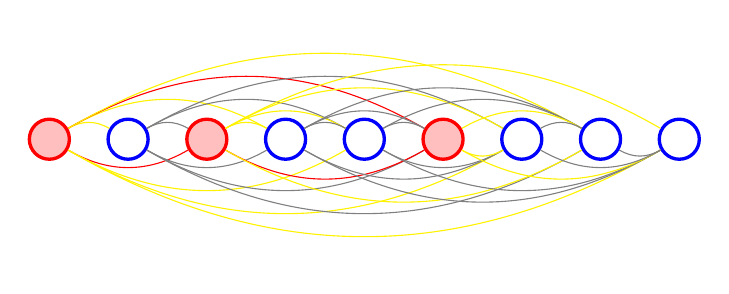
\begin{tikzpicture}
\node[on,text width=0.35cm](0){};
\node[off,text width=0.35cm,right of = 0](1){};
\node[on,text width=0.35cm,right of = 1](2){};
\node[off,text width=0.35cm,right of = 2](3){};
\node[off,text width=0.35cm,right of = 3](4){};
\node[on,text width=0.35cm,right of = 4](5){};
\node[off,text width=0.35cm,right of = 5](6){};
\node[off,text width=0.35cm,right of = 6](7){};
\node[off,text width=0.35cm,right of = 7](8){};
\path (0) edge[bend left,color=yellow] (1);
\path (0) edge[bend right,color=red] (2);
\path (0) edge[bend left,color=yellow] (3);
\path (0) edge[bend right,color=yellow] (4);
\path (0) edge[bend left,color=red] (5);
\path (0) edge[bend right,color=yellow] (6);
\path (0) edge[bend left,color=yellow] (7);
\path (0) edge[bend right,color=yellow] (8);
\path (1) edge[bend left,color=gray] (2);
\path (1) edge[bend right,color=gray] (3);
\path (1) edge[bend left,color=gray] (4);
\path (1) edge[bend right,color=gray] (5);
\path (1) edge[bend left,color=gray] (6);
\path (1) edge[bend right,color=gray] (7);
\path (2) edge[bend left,color=yellow] (3);
\path (2) edge[bend left,color=yellow] (4);
\path (2) edge[bend right,color=red] (5);
\path (2) edge[bend left,color=yellow] (6);
\path (2) edge[bend right,color=yellow] (7);
\path (2) edge[bend left,color=yellow] (8);
\path (3) edge[bend left,color=gray] (4);
\path (3) edge[bend left,color=gray] (5);
\path (3) edge[bend right,color=gray] (6);
\path (3) edge[bend left,color=gray] (7);
\path (3) edge[bend right,color=gray] (8);
\path (4) edge[bend left,color=gray] (5);
\path (4) edge[bend right,color=gray] (6);
\path (4) edge[bend left,color=gray] (7);
\path (4) edge[bend right,color=gray] (8);
\path (5) edge[bend right,color=yellow] (6);
\path (5) edge[bend left,color=yellow] (7);
\path (5) edge[bend right,color=yellow] (8);
\path (6) edge[bend left,color=gray] (7);
\path (6) edge[bend right,color=gray] (8);
\path (7) edge[bend right,color=gray] (8);
\end{tikzpicture}
\end{center}
\caption{Learning in the associate network. The pattern has been imposed and connection strengths are changed. The red links increase by $\eta(1-\alpha)^2$ and the gray by $\eta(-\alpha)^2$, the yellow links decrease by $\eta \alpha(1-\alpha)$.\label{fig:hebb}}
\end{figure}

During recall some of the neurons are held in the active state and the
rest of the network evolves according to a threshold input rule. That
means each neuron has an input given by
\begin{equation}
r_i=\sum{w_{ij}x_j}
\end{equation}
and is set in the active state if $r_i>0$. The idea is that after
learning the pattern $\{0,2,5\}$
\begin{center}
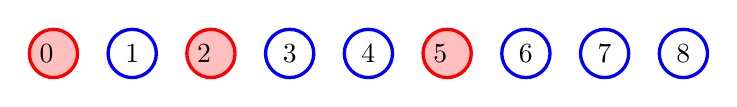
\begin{tikzpicture}
\node[on,text width=0.35cm](0){0};
\node[off,text width=0.35cm,right of = 0](1){1};
\node[on,text width=0.35cm,right of = 1](2){2};
\node[off,text width=0.35cm,right of = 2](3){3};
\node[off,text width=0.35cm,right of = 3](4){4};
\node[on,text width=0.35cm,right of = 4](5){5};
\node[off,text width=0.35cm,right of = 5](6){6};
\node[off,text width=0.35cm,right of = 6](7){7};
\node[off,text width=0.35cm,right of = 7](8){8};
\end{tikzpicture}
\end{center}
the connections between these nodes will be strong, so if the network has nodes $\{0,5\}$ activated
\begin{center}
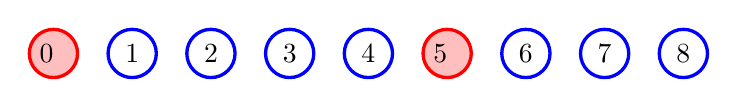
\begin{tikzpicture}
\node[on,text width=0.35cm](0){0};
\node[off,text width=0.35cm,right of = 0](1){1};
\node[off,text width=0.35cm,right of = 1](2){2};
\node[off,text width=0.35cm,right of = 2](3){3};
\node[off,text width=0.35cm,right of = 3](4){4};
\node[on,text width=0.35cm,right of = 4](5){5};
\node[off,text width=0.35cm,right of = 5](6){6};
\node[off,text width=0.35cm,right of = 6](7){7};
\node[off,text width=0.35cm,right of = 7](8){8};
\end{tikzpicture}
\end{center}
the value $r_{2}=w_{12}+w_{52}$ will be larger than the threshold and
the subsequent dynamics will switch neuron 2 on. However, in this
network, if a different initial set of neurons are activated, the
activity will die away because the $r_i$ will all be sub-threshold.

When many patterns are stored it is likely that there will be
interference between them. This is illustrated in
Fig.~\ref{fig:interfere}. Although the figure shows how a single
neuron fails to participate in two patterns, for larger networks some
overlap is possible, but too much overlap prevents retrieval. In fact
the capacity is proportional to the number of neurons, $N$. A
hand-waving argument goes like this: the number of connections is
roughly $N^2$ and the amount of information in a pattern is $N$ so the
number of patterns that can be stored is $N^2/N=N$ \cite{Amit1992a}.


\begin{figure}
\begin{center}
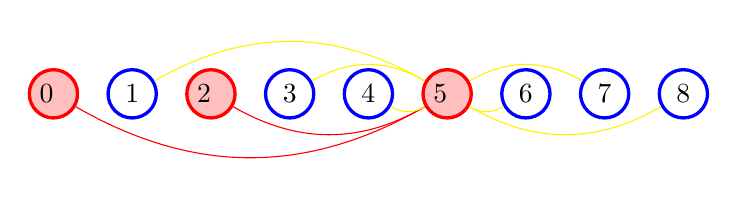
\begin{tikzpicture}
\node[on,text width=0.35cm](0){0};
\node[off,text width=0.35cm,right of = 0](1){1};
\node[on,text width=0.35cm,right of = 1](2){2};
\node[off,text width=0.35cm,right of = 2](3){3};
\node[off,text width=0.35cm,right of = 3](4){4};
\node[on,text width=0.35cm,right of = 4](5){5};
\node[off,text width=0.35cm,right of = 5](6){6};
\node[off,text width=0.35cm,right of = 6](7){7};
\node[off,text width=0.35cm,right of = 7](8){8};
\path (5) edge[bend left,color=red] (0);
\path (5) edge[bend right,color=yellow] (1);
\path (5) edge[bend left,color=red] (2);
\path (5) edge[bend right,color=yellow] (3);
\path (5) edge[bend left,color=yellow] (4);
\path (5) edge[bend right,color=yellow] (6);
\path (5) edge[bend left,color=yellow] (7);
\path (5) edge[bend right,color=yellow] (8);
\end{tikzpicture}
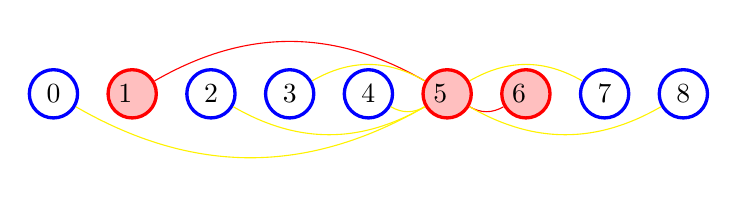
\begin{tikzpicture}
\node[off,text width=0.35cm](0){0};
\node[on,text width=0.35cm,right of = 0](1){1};
\node[off,text width=0.35cm,right of = 1](2){2};
\node[off,text width=0.35cm,right of = 2](3){3};
\node[off,text width=0.35cm,right of = 3](4){4};
\node[on,text width=0.35cm,right of = 4](5){5};
\node[on,text width=0.35cm,right of = 5](6){6};
\node[off,text width=0.35cm,right of = 6](7){7};
\node[off,text width=0.35cm,right of = 7](8){8};
\path (5) edge[bend left,color=yellow] (0);
\path (5) edge[bend right,color=red] (1);
\path (5) edge[bend left,color=yellow] (2);
\path (5) edge[bend right,color=yellow] (3);
\path (5) edge[bend left,color=yellow] (4);
\path (5) edge[bend right,color=red] (6);
\path (5) edge[bend left,color=yellow] (7);
\path (5) edge[bend right,color=yellow] (8);
\end{tikzpicture}
\end{center}
\caption{Interference in an associate network. Neuron 5 is involved in two patterns and, as a consequence, some of its connections are strengthen for one pattern and weakened for the other, if these strengthening and weakening effects are similar in size it makes it unlikely that either pattern will be accurately retrieved.\label{fig:interfere}}
\end{figure}


The capacity is also larger if there is sparseness; one way to think
of this is to observe the weight decrease between an active and
inactive connection is $\delta w_{ij}=-\eta \alpha (1-\alpha)$ so the
smaller $\alpha$ is the smaller the amount these links are
decreased. Links are decreased if, in the pattern, one neuron is
active and one inactive, they are strengthened if both neurons are
active, the increase is $\eta (1-\alpha)^2$. Hence, it takes of the
order of $1/\alpha$ patterns where a connection is weakened to wipe
out the strengthening that results if the connection is part of a
pattern. In fact, it is estimated that the capacity of a network is
\begin{equation}
P=\frac{k}{\alpha}N
\end{equation}
where $k$ is constant which has been found to be about $k\approx
0.035$, this is reduced to 
\begin{equation}
P=c\frac{k}{\alpha}N
\end{equation}
if there are missing connections, where $c$ stands for the fraction of pairs that are connected.

The actual sparseness of the brain needs to balance this advantage,
the increased capacity, along with a metabolic advantage and more
abstract computational advantage which says that a sparse coding for
information involves object recognition or segmentation against the
disadvantages, most obviously the vulnerability of the pattern to the
loss of neurons or connections and, perhaps more importantly, a sparse
code involves fewer elements and so may be less useful for
retrieval. It is hard to actually estimate sparseness in practice
since neurons are not, in reality, on-off units.

\begin{thebibliography}{10}

\bibitem{McCullochPitts1943}
McCulloch, W and Pitts, W. (1943). A logical calculus of the ideas immanent in nervous activity. 
\newblock Bulletin of Mathematical Biophysics, 5:115--133. 

\bibitem{Rosenblatt1958}
Rosenblatt, F. (1958), The Perceptron: A Probabilistic Model for Information Storage and Organization in the Brain, Cornell Aeronautical Laboratory.
\newblock Psychological Review, 65:386--408.

\bibitem{Albus1971a}
Albus, JS. (1971) A theory of cerebellar function. 
\newblock Mathematical Biosciences 10: 25--61.


\bibitem{GaoEtAl1996a}
Gao J-H, Parsons LM, Bower JM, Xiong J, Li J and Fox PT (1996) Cerebellum implicated in sensory acquisition and discrimination rather than motor control.
\newblock Science 272: 545--7. 

\bibitem{Marr1969a}
Marr, D (1969) A theory of cerebellar cortex.
\newblock Journal of Physiology 202: 437--70.

\bibitem{Hopfield1982}
Hopfield, JJ. (1982) Neural networks and physical systems with emergent collective computational abilities.
\newblock Proceedings of the National Academy of Sciences of the USA, 79:2554--2558.

\bibitem{Hebb1949a}
Hebb DO. (1949) The Organization of Behavior. 
\newblock New York: Wiley \& Sons.


\bibitem{Amit1992a} Amit D. (1992) Modeling Brain Function: The World
  of Attractor Neural Networks.
\newblock Cambridge University Press, Cambridge England.


\end{thebibliography}

\end{document}

